\section{Introduction:}

The diode analysis will now be expanded to include time-varying functions such as
the sinusoidal waveform and the square wave. There is no question that the degree of
difficulty will increase, but once a few fundamental maneuvers are understood, the
analysis will be fairly direct and follow a common thread.

\subsection{Half-Wave Rectification:}

Over one full cycle, defined by the period {\bfseries\itshape T} of Figure 2.1.0, the average value (the
algebraic sum of the areas above and below the axis) is zero. The circuit of Figure 2.1.0,
called a {\bfseries\itshape half-wave rectifier}, will generate a waveform $V_{o}$ that will have an average
value of particular, use in the ac-to-dc conversion process. When employed in the rectification
process, a diode is typically referred to as a rectifier. Its power and current
ratings are typically much higher than those of diodes employed in other applications,
such as computers and communication systems.

\begin{multicols}{2}
\begin{figure}[H]
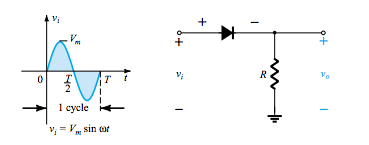
\includegraphics[scale=.7]{Half-Wave.png}
\centering \linebreak \linebreak Figure 2.1.0: Half-Wave Rectifier.
\end{figure}

During the interval {\bfseries\itshape t} = 0 $\rightarrow \frac{T}{2}$ in Figure 2.1.0  the polarity of the applied voltage $V_{i}$ is such as to establish "pressure" in the direction indicated and turn on the diode with
the polarity appearing above the diode. Substituting the short-circuit equivalence for
the ideal diode will result in the equivalent circuit of Figure 2.1.1, where it is fairly obvious
that the output signal is an exact replica of the applied signal. The two terminals
defining the output voltage are connected directly to the applied signal via the
short-circuit equivalence of the diode.
\end{multicols}

\begin{figure}[H]
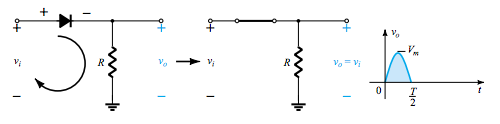
\includegraphics[scale=.8]{Conduction.png}
\centering \linebreak \linebreak Figure 2.1.1: Conduction Region ( 0 $\rightarrow \frac{T}{2}$ ).
\end{figure}

For the period $\frac{T}{2} \rightarrow T$, the polarity of the input $V_{i}$ is as shown in Figure 2.1.2 and
the resulting polarity across the ideal diode produces an “off” state with an open-circuit
equivalent. The result is the absence of a path for charge to flow and $V_{o}$ = {\bfseries\itshape iR} =
{\bfseries\itshape (0)R} = 0 V for the period $\frac{T}{2} \rightarrow T$. The input $V_{i}$ and the output $V_{o}$ were sketched together in Figure 2.1.3 for comparison purposes. The output signal $V_{o}$ now has a net positive
area above the axis over a full period and an average value determined by:

\begin{equation}
V_{dc} = 0.318 V_{m}
\end{equation}

\begin{figure}[H]
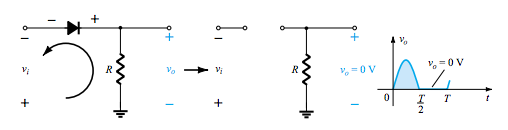
\includegraphics[scale=.8]{Nonconduction.png}
\centering \linebreak \linebreak Figure 2.1.2: Non-conduction region  ( $\frac{T}{2} \rightarrow T$ ).
\end{figure}

\begin{multicols}{2}
\begin{figure}[H]
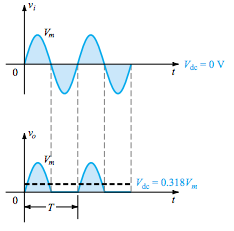
\includegraphics[scale=.6]{Half-Wave-Rectified-Signal.png}
\centering \linebreak \linebreak Figure 2.1.3: Half-wave rectified signal.
\end{figure}

The process of removing one-half the input signal to establish a dc level is aptly
called {\bfseries\itshape half-wave rectification.}
\end{multicols}

\subsection{Full-Wave Rectification:}

\subsubsection{Bridge Network:}

The dc level obtained from a sinusoidal input can be improved $100 \%$ using a process
called {\bfseries\itshape full-wave rectification.} The most familiar network for performing such a function 
appears in Figure 2.2.1.0 with its four diodes in a bridge configuration. During the
period t = 0 to $\frac{T}{2}$ the polarity of the input is as shown in Figure 2.2.1.1.The resulting polarities across the ideal diodes are also shown in Figure 2.2.1.1 to reveal that $D_{2}$ and $D_{3}$
are conducting while $D_{1}$ and $D_{4}$ are in the “off” state. The net result is the configuration
of Figure 2.2.1.2, with its indicated current and polarity across {\bfseries\itshape R}. Since the diodes
are ideal the load voltage is $V_{o} = V_{i}$, as shown in the same figure.

\begin{multicols}{2}
\begin{figure}[H]
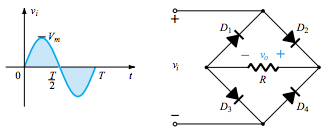
\includegraphics[scale=.6]{Full-wave-bridge-rectifier.png}
\centering \linebreak \linebreak Figure 2.2.1.0: Full-wave bridge rectifier.
\end{figure}

\begin{figure}[H]
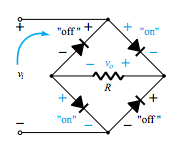
\includegraphics[scale=.6]{bridge.png}
\centering \linebreak \linebreak Figure 2.2.1.1: Network of Figure 2.2.1.0 for the period $0 \rightarrow \frac{T}{2}$ of the input voltage $V_{i}$.
\end{figure}
\end{multicols}

\begin{figure}[H]
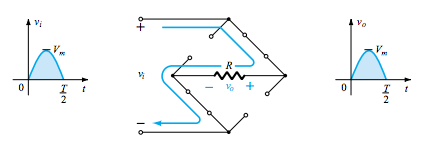
\includegraphics[scale=1]{path.png}
\centering \linebreak \linebreak Figure 2.2.1.2: Conduction path for the positive region of $V_{i}$.
\end{figure}

For the negative region of the input the conducting diodes are $D_{1}$ and $D_{4}$, resulting
in the configuration of Figure 2.2.1.3. The important result is that the polarity across
the load resistor {\bfseries\itshape R} is the same as in Figure 2.2.1.1, establishing a second positive pulse,
as shown in Figure 2.2.1.3. Over one full cycle the input and output voltages will appear
as shown in Figure 2.2.1.4.

\begin{figure}[H]
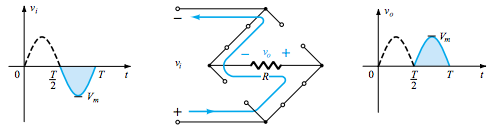
\includegraphics[scale=1]{negative.png}
\centering \linebreak \linebreak Figure 2.2.1.3: Conduction path for the negative region of $V_{i}$.
\end{figure} \hfill

\begin{multicols}{2}
\begin{figure}[H]
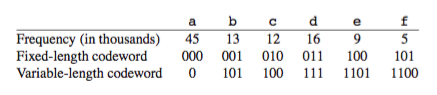
\includegraphics[scale=.68]{1.png}
\centering \linebreak \linebreak Figure 2.2.1.4: Input and output waveforms for a full-wave rectifier.
\end{figure}

Since the area above the axis for one full cycle is now twice that obtained for a
half-wave system, the dc level has also been doubled:

\begin{ceqn}
\begin{align}
V_{dc} = 0.636V_{m}
\end{align}
\end{ceqn} 
\end{multicols}

\subsubsection{Center-Tapped Transformer:}

A second popular full-wave rectifier appears in Figure 2.2.2.0 with only two diodes but
requiring a center-tapped (CT) transformer to establish the input signal across each
section of the secondary of the transformer. During the positive portion of $V_{i}$ applied
to the primary of the transformer, the network will appear as shown in Figure 2.2.2.1. $D_{1}$
assumes the short-circuit equivalent and $D_{1}$ the open-circuit equivalent, as determined
by the secondary voltages and the resulting current directions. The output voltage appears
as shown in Figure 2.2.2.1.

\begin{multicols}{2}
\begin{figure}[H]

\includegraphics[scale=.53]{2.png}
\centering \linebreak \linebreak Figure 2.2.2.0: Center-tapped transformer full-wave rectifier.
\end{figure}

\begin{figure}[H]
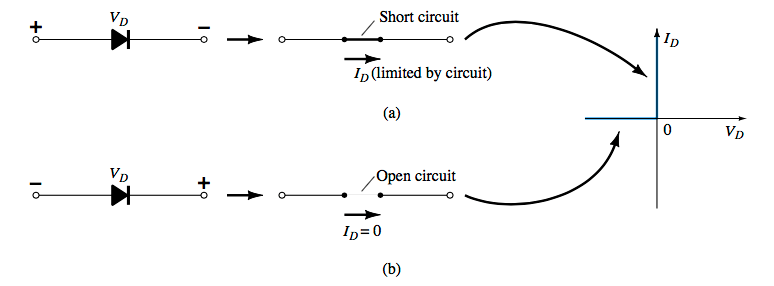
\includegraphics[scale=.58]{3.png}
\centering \linebreak \linebreak Figure 2.2.2.1: Network conditions for the positive region of $V_{i}$.
\end{figure}
\end{multicols}

\begin{multicols}{2}
During the negative portion of the input the network appears as shown in Figure 2.2.2.2, reversing the roles of the diodes but maintaining the same polarity for the voltage across the load resistor {\bfseries\itshape R}. The net effect is the same output as that appearing in Figure 2.2.1.4 with the same dc levels.

\begin{figure}[H]
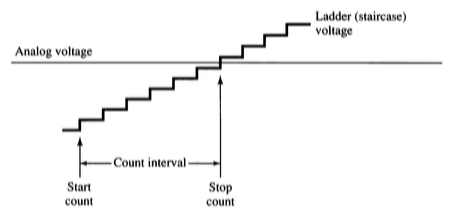
\includegraphics[scale=.58]{4.png}
\centering \linebreak \linebreak Figure 2.2.2.2: Network conditions for the negative region of $V_{i}$.
\end{figure}
\end{multicols}

\pagebreak